\documentclass{article}

\usepackage{graphicx}
\usepackage{tikz}
\usepackage{tikzsymbols}
\usetikzlibrary{calc,patterns,shapes.geometric}
\pagestyle{empty}
\usepackage[margin=0pt]{geometry}
\geometry{papersize={14in,12in}}

\def\centerarc[#1](#2)(#3:#4:#5){\draw[#1] ($(#2)+({#5*cos(#3)},{#5*sin(#3)})$) arc (#3:#4:#5);}

\begin{document}
	\begin{figure}
		\centering
		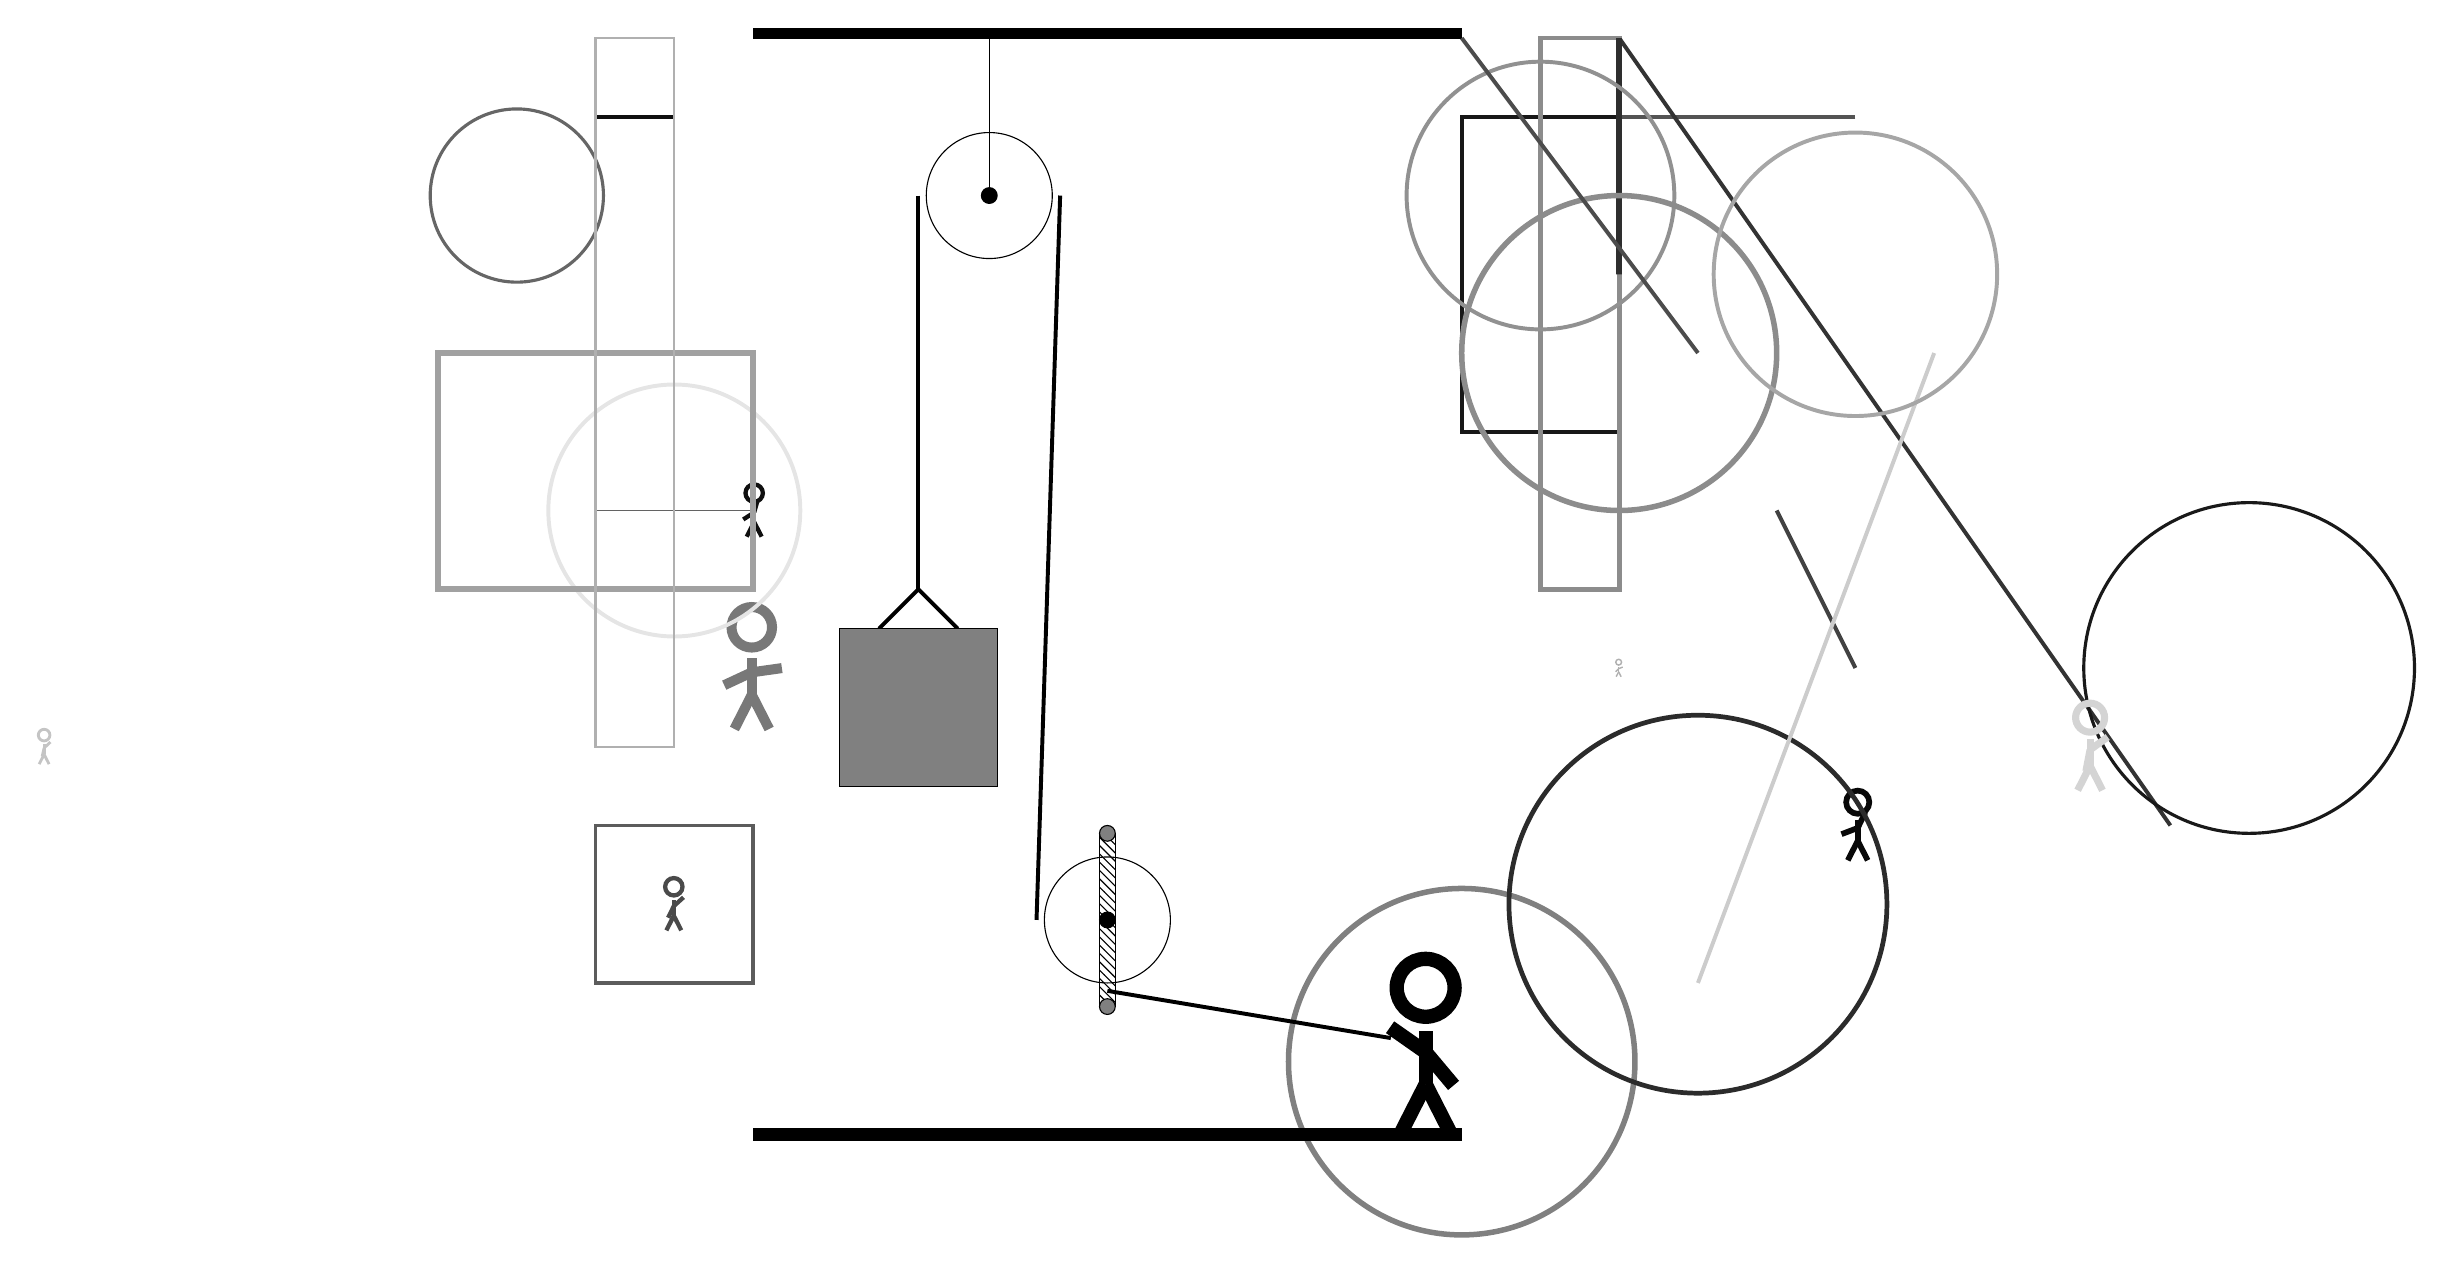
\begin{tikzpicture}
			%%%%% START %%%%%
			
			\draw[fill=black] (-2, 14) rectangle (7, 14.125);
			
			\draw (1, 12) circle (0.8);
			\draw[fill=black] (1, 12) circle (0.1);
			\draw (1, 14) -- (1, 12);
			
			\draw[fill=white](2.5, 2.8) circle (0.8);
			\draw[fill=black] (2.5, 2.8) circle (0.1);
			\draw[pattern=north west lines, pattern color=black] (2.4, 3.9) rectangle (2.6, 1.7);
			\draw[fill=black!50] (2.5, 3.9) circle (0.1);
			\draw[fill=black!50] (2.5, 1.7) circle (0.1);
			
			\draw[line width=0.5mm] (-0.4, 6.5) -- (0.1, 7.0) -- (0.6, 6.5);
			\draw[fill=black!50] (-0.9, 6.5) rectangle (1.1, 4.5);
			
			\draw [line width=0.4mm, color=black!60](-5, 12) circle (1.1);
			
			\draw[line width=0.5mm, color=black!67](12, 13) -- (9, 13);
			\node[line width=0.5mm, color=black!97] at (12, 4) {\Strichmaxerl[4][21][64]};
			\draw[line width=0.5mm, color=black!80](9, 14) -- (16, 4);
			
			\node[line width=0.2mm, color=black!53] at (-2, 6) {\Strichmaxerl[7][25][8]};
			\draw[line width=0.5mm, color=black!91] (9, 13) rectangle (7, 9);
			\draw[line width=0.5mm, color=black!74](12, 6) -- (11, 8);
			\node[line width=0.6mm, color=black!94] at (-2, 8) {\Strichmaxerl[3][33][74]};
			\draw [line width=0.4mm, color=black!90](17, 6) circle (2.1);
			\draw[line width=0.5mm, color=black!94](-3, 13) -- (-4, 13);
			\node[line width=0.6mm, color=black!71] at (-3, 3) {\Strichmaxerl[3][64][42]};
			\draw[line width=0.2mm, color=black!61] (-2, 8) rectangle (-4, 10);
			\draw [line width=0.7mm, color=black!50](7, 1) circle (2.2);
			
			\draw[line width=0.6mm, color=black!45] (8, 14) rectangle (9, 7);
			\draw[line width=0.7mm, color=black!82] (9, 11) rectangle (9, 14);
			\draw [line width=0.6mm, color=black!83](10, 3) circle (2.4);
			
			\node[line width=0.4mm, color=black!17] at (15, 5) {\Strichmaxerl[5][79][36]};
			\draw [line width=0.5mm, color=black!10](-3, 8) circle (1.6);
			\node[line width=0.5mm, color=black!31] at (9, 6) {\Strichmaxerl[1][46][20]};
			\draw[line width=0.4mm, color=black!64] (-2, 4) rectangle (-4, 2);
			\draw [line width=0.5mm, color=black!43](8, 12) circle (1.7);
			\draw[line width=0.5mm, color=black!20](10, 2) -- (13, 10);
			
			\draw [line width=0.7mm, color=black!45](9, 10) circle (2.0);
			\draw [line width=0.5mm, color=black!35](12, 11) circle (1.8);
			\draw[line width=0.7mm, color=black!37] (-2, 7) rectangle (-6, 10);
			\node[line width=0.6mm, color=black!23] at (-11, 5) {\Strichmaxerl[2][77][43]};
			\draw[line width=0.5mm, color=black!70](7, 14) -- (10, 10);
			\draw[line width=0.3mm, color=black!31] (-4, 5) rectangle (-3, 14);
			
			
			\draw[line width=0.5mm] (0.1, 12) -- (0.1, 7.0);
			\centerarc[line width=0.5mm](1, 12)(0:180:0.9);
			\draw[line width=0.5mm](1.9, 12) -- (1.6, 2.8);
			\centerarc[line width=0.5mm](2.5, 2.8)(180:270:0.9);
			\draw[line width=0.5mm](2.5, 1.9) -- (6.1, 1.3);
			
			\node at (6.5, 1.2) {\Strichmaxerl[10][-35][-50]};
			
			\draw[fill=black] (-2, 0) rectangle (7, 0.15);
			
			%%%%% END %%%%%
		\end{tikzpicture}
	\end{figure}	
\end{document}